\documentclass[12pt]{article}
\usepackage{amsmath}
\usepackage{amsfonts}
\usepackage{amssymb}
\usepackage{graphicx}
\usepackage{subfigure}
\usepackage[top=.9in,left = 0.9in, bottom = .9in, right = .9in]{geometry}
\newcommand*{\plogo}{\fbox{$\mathcal{KHP}$}} % Generic publisher logo

%----------------------------------------------------------------------------------------
%	TITLE PAGE
%----------------------------------------------------------------------------------------

\newcommand*{\titleGP}{\begingroup % Create the command for including the title page in the document
\centering % Center all text
\vspace*{\baselineskip} % White space at the top of the page

\rule{\textwidth}{1.6pt}\vspace*{-\baselineskip}\vspace*{2pt} % Thick horizontal line
\rule{\textwidth}{0.4pt}\\[\baselineskip] % Thin horizontal line

{\LARGE Image Feature Extraction for Plankton Classification}\\[0.2\baselineskip] % Title

\rule{\textwidth}{0.4pt}\vspace*{-\baselineskip}\vspace{4pt} % Thin horizontal line
\rule{\textwidth}{1.6pt}\\[\baselineskip] % Thick horizontal line

\scshape % Small caps
An exploration of image feature extraction and classification on \\ large oceanographic data\\[\baselineskip] % Tagline(s) or further description
May 12, 2015\par % Location and year

\vspace*{2\baselineskip} % Whitespace between location/year and editors

Authors \\[\baselineskip]
{\Large NICK HOCKENSMITH \\ KEVIN PARK \\ DANE SKINNER\par} % Editor list
{\itshape Oregon State University \\ Corvallis\par} % Editor affiliation

\vfill % Whitespace between editor names and publisher logo

\plogo \\[0.3\baselineskip] % Publisher logo
{\scshape 2015} \\[0.3\baselineskip] % Year published
{\large KIDDER HALL PRESS}\par % Publisher

\endgroup}

%----------------------------------------------------------------------------------------
%	BLANK DOCUMENT
%----------------------------------------------------------------------------------------

\begin{document} 

\pagestyle{empty} % Removes page numbers

\titleGP % This command includes the title page

%---------------------------------------------------
%	TABLE OF CONTENTS
%---------------------------------------------------
\newpage
\tableofcontents

%---------------------------------------------------
%	INTRODUCTION
%---------------------------------------------------
\newpage
\pagestyle{plain}
\section{Introduction}
Plankton, perhaps surprisingly, form a critical link in the global ecosystem and are a fundamental source of food and energy for aquatic wildlife. As such, the population levels of plankton are an ideal metric for determining the health and viability of oceans and aquatic ecosystems. The challenge thus becomes determining the best way to classify and count the multitude of phytoplankton and zooplankton species from a sample of ocean water.  Modern imaging systems can easily produce hundreds of thousands of images in a short time scale, so using human based means is daunting and often of minimal utility. \\

\noindent To address this challenge, we each explored a different method of image feature extraction followed by a different approach of test data classification.  N. Hockensmith used image moments to extract features from images and built the classification model using the random forest algortihm. K. Park used a histogram method for feature extraction followed by random forest classification. Finally, D. Skinner extracted feature vectors using an R command from the company Indico, classifying these vectors via the K-Nearest Neighbors algorithm. 


%---------------------------------------------------
%   Image Feature Extraction: 
%--------------------------------------------------- 
\section{Feature Extraction}
The most difficult task in image classification is extracting information (features) from the images. The different species of plankton come in varying shapes and sizes. Classification is further complicated by the varying quality of the images as well as the heterogeneity in pixel resoltuion. The literature on image processing is broad in scope, and the proposed methods of feature extraction can be quite complicating. Some of the more complicated methods are SIFT, SURF, Bag of Features, etc. However, for the purposes of this report, image features will be extracted using \textit{Krawtchouk} moments and the \textit{Histogram} method. Both methods were found to have performed better than ``best guess" criteria as reported on Kaggle's National Data Science Competition board. Additionally, features were also obtained using a more complex image extraction package available on R.

\subsection{Krawtchouk Moments}
Krawtchouk moments belong to the broader class of discrete, orthogonal moments. The ($m+n$) Krawtchouk moment itself is defined as the sum, over the x-y coordiantes, of the product of the pixel intensity function of the image $f(x,y)$ and two weighted Krawtchouk polynomials ($K_n(a;p,N$), $a\in \{x,y\}$ and $n\in \mathbb{N}$ is order of the moment in the x- or y-direction) where each ploynomial is specified in either the x-direction or the y-direction. The equation is provided below.
\begin{equation*}
Q_{nm} = \sum_{x=0}^{N-1}\sum_{y=0}^{M-1}\bar{K}_n(x;p_1,N-1)\bar{K}_m(y;p_2,M-1)f(x,y),
\end{equation*}
The motivation behind choosing to use Krawtchouk moments for the project is two-fold. First, they appear to be popular in the literture for their ability to reconstruct images at lower orders of moments. Second, their orthogonal properties make them invariant to scaling, translation, and rotation. For simplicity, only moments of order ($n+n$) will be considered. The optimal order was determined by comparing the classification error across the different moments. As you can see below, moments of order $5$ through $22$ and thir respective correct classification percentages are provided. Observe that model performance begins to plateau after the $15^{th}$ moment.
\begin{figure}[h]
	\begin{center}	
		\subfigure[Moment ]{
			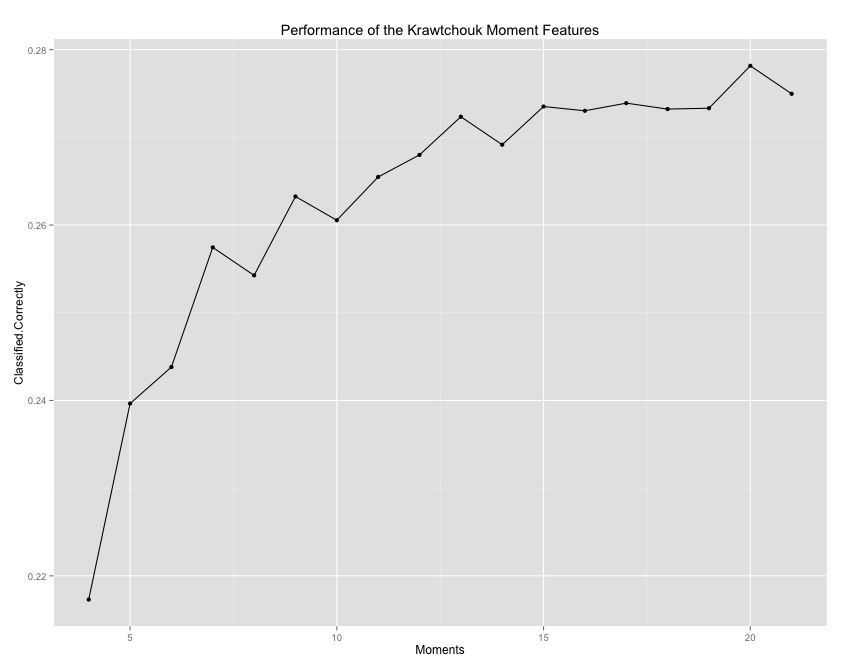
\includegraphics[scale=0.35]{PerfPlot.jpeg}}
	\end{center}
\end{figure} 

\subsection{Histogram Method}
The histogram method extracts information from the distribution of gray scale values that make up the image. We simply segmented the color ranges into bins and counted the frequency of values within each bin. 
\begin{figure}[h]
	\begin{center}
	\subfigure[Plankton]{
		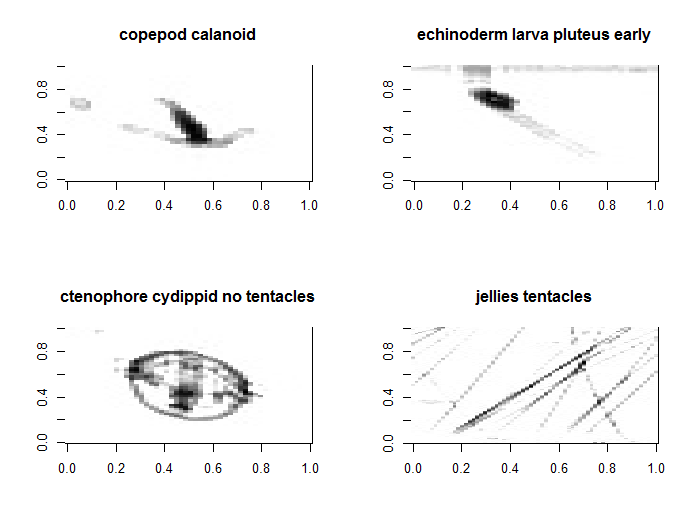
\includegraphics[scale=0.3]{images.png}}
	\subfigure[Grayscale Density]{
		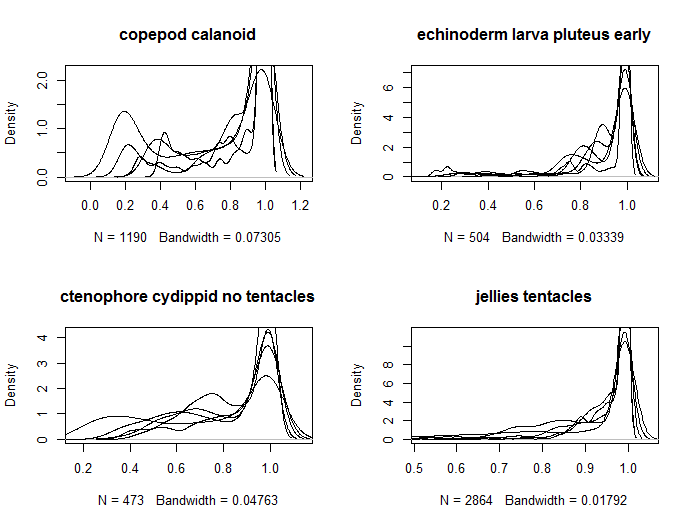
\includegraphics[scale=0.3]{grayscale.png}}
	\end{center}
\end{figure}
Notice in the density plots for the species Copepod Calanoid and Ctenophore Cydipid (no tentacles)  provided above that the distribution of values on the grey-scale are distinct. Note that values were scaled down to the interval $[0,1]$. In general, this will usually be the case because of the uniqueness in the size and shape of the various species of plankton. $10$ features total were extracted from each image, each feature representing one bin on the unit interval (with a bin-width of 0.1).
	
%---------------------------------------------------
%    Results from classificaiton models 
%---------------------------------------------------
\section{Classification Models}

Two methods for classification, and their results, are provided below. The first method used the Random Forest and the second method the K-Nearest Neighbors algorithm. 

\subsection{Random Forest}
%\begin{figure}[h]
%	\begin{center}
%		\subfigure[Histogram Features]{
%			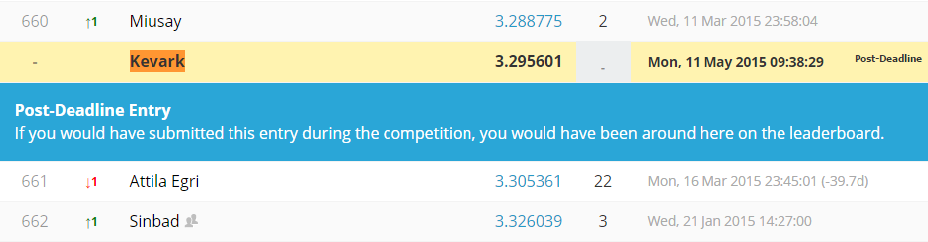
\includegraphics[scale=0.3]{submission.png}}
%		\subfigure[Combined feature extraction]{
%			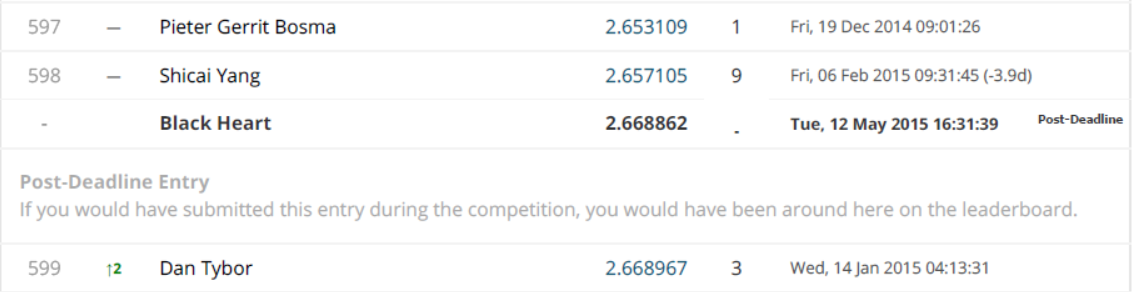
\includegraphics[scale=0.3]{combined.png}}
%	\end{center}
%\end{figure}
The random forest procedure was implemented, setting the number of trees for each model fitting to $500$. Kaggle scores were obtained from fitting models for the Krawtchouck and Histogram methods individually. For the \textit{Krawtchouk} moments, the $10^{th}$-order moment obtained a score of 3.67 (714 out of 1049) and the $22^{nd}$-order moment received a score of 3.54 (704 out of 1049). Even though the $22^{nd}$-order model performed better, the model benefited marginally from the addition of the $384$ additional features. The histogram method received a score of 3.29 (660 out of 1049). Pooling features from both methods provided a significant boost in precision. The combination of the $9^{th}$-order moments with the $10$-bin features yields a score of 2.66 (598 out of 1049). This was our best result under the current timeframe of the project.

\subsection{K-Nearest Neighbors}

The K-Nearest Neighbors algorithm was a logical choice for classification of plankton because the algorithm is simple to impement and can provide as a benchmark for further classification. The algorithm works by assigning classes to images in the test set based on the Euclidean distance between images in the training set. \\

\noindent R does not contain much in the way of built-in image extraction features, but it does contain the command \textsf{image\_{features}} in the \textsf{indicoio} package.  This command produces a sparse, 2048 digit feature vector for each image that can then be used to calculate the Eucliden distances between different feature vectors. The drawbacks of this approach for feature extraction includes the production of possibly ``too much" data to be reasonably useful and would likely require several more time intensive steps of data preparation for variable reduction. \\

\noindent The first few attempts at implementing the k-NN algorithm revealed some critical issues. One such issue is the choice in the number of nearest neighbors to use. Too few neighbors resulted in images being classified to different groups with equal probabilities. Kaggle consequently counts this is an incorrect classification.  Another challenge is the susceptibility of the k-NN algorithm to noise and unimportant variables.  As mentioned before, the feature vector is likely too large. Because of this, there is a reasonable chance that k-NN is suffering from too many variables. Currently, the best Kaggle score received for this approach is above the benchmark score.  

%---------------------------------------------------
%	FUTURE WORK
%---------------------------------------------------
\newpage
\section{Discussion and Future Work}
In summary, the basic feature extraction methods decribed in this report do provide crucial information for the classification of plankton, as demonstrated with Kaggle scores above the ``random chance" threshold. However, these methods are far from perfect in classifying plankton. In addition, using a large feature extraction algorithm, such as the \textsf{indico.io} package, doesn't necessarly mean the prouction of more features will build a better model. \\

\noindent Future work would include further refinements to both the classification algorithms and the extraction of image features with the goal of reducing misclassification as much as possible. Also, attempting other classification algorithms (Neuaral Networks, Naive Bayes, etc.) would also be a prime area to explore, but as always, ever expanding computation time cannot be ignored.

\section{References}
	\begin{enumerate}
		\item Yap, Paramesran, and Ong, \textit{Image Analysis by Krawtchouk Moments}, IEEE Transactions on Image Processing, Vol. 12, No. 11, November 2003
		\item Rani and Devaraj, \textit{Face recognition using Krawtchouk moment}, Sadhana, Vol. 37, Part 4, August 2012, pp. 441–460
	\end{enumerate}
\end{document}
